\documentclass[10pt]{article}
\usepackage{float}
\RequirePackage{eso-pic}
\usepackage{caption}
\captionsetup[table]{labelformat=empty}



\usepackage{geometry}
\geometry{
a4paper,
left=11mm,
right=14mm,
top=37mm,
bottom=14mm,
}



\usepackage{colortbl}
\usepackage{fontspec}
\setmainfont[Ligatures=TeX]{Calibri}



\newcommand\BackgroundPic{%
\put(0,0){%
\parbox[b][\paperheight]{\paperwidth}{%
\vfill
\centering
\includegraphics{MBIE_generic_background.pdf}%
\vfill
}}}



\begin{document}
\thispagestyle{empty}
\AddToShipoutPicture{\BackgroundPic}
\section*{Key Export Statistics\footnotemark - Bovine Meat\footnotemark }
Published on April 11, 2016. \par
\small{\noindent{\textit{Monthly data from January 2000 to November 2015.}}}
\begin{table}[ht]
\centering
{\scriptsize
\begin{tabular}[t]{p{1.8cm}>{\hfill}p{1.4cm}>{\hfill}p{1.4cm}>{\hfill}p{1.6cm}>{\hfill}p{1.9cm}>{\hfill}p{2cm}>{\hfill}p{1.9cm}>{\hfill}p{1.5cm}}
 \textbf{Country} & \textbf{Yearly Qty} & \textbf{Yearly Value} & \textbf{Yearly Price} & \textbf{3Year CAGR(Qty)} & \textbf{3Year CAGR(Value)} & \textbf{3Year CAGR(Price)} & \textbf{Price Elasticity} \\
\hline
USA & 2,595 & 50.4 & \$19.4 & -9.3\% & -5.8\% & 3.8\% & -2.4 \\  
Australia & 4,230 & 32.2 & \$7.6 & 5.8\% & 2\% & -3.6\% & -1.6 \\  
Japan & 905 & 7.7 & \$8.5 & -6.3\% & -10.4\% & -4.4\% & 1.4 \\  
Philippines & 661 & 7.5 & \$11.4 & 4.5\% & 14.4\% & 9.5\% & 0.5 \\  
South Korea & 1,727 & 5.5 & \$3.2 & 8.1\% & 11.8\% & 3.4\% & 2.4 \\  
Tonga & 347 & 3.2 & \$9.3 & -2.6\% & -0.3\% & 2.3\% & -1.1 \\  
Other & 2,523 & 25.2 & \$10.0 & 3.6\% & 7.2\% & 3.5\% & 1.0 \\  
Total & 12,987 & 131.7 & \$10.1 & 0.7\% & -0.6\% & -1.2\% & -0.5 \\  
\hline
\end{tabular}
}
\caption{\scriptsize Top 6 Bovine Meat Markets for year ending November - 2015: Quantity('000 kg) Value(NZ\$Mill), Price and their last 3-Year Growth Rates}
\end{table}


\vspace{-0.7cm}



   \begin{figure}[H]
   \centering
    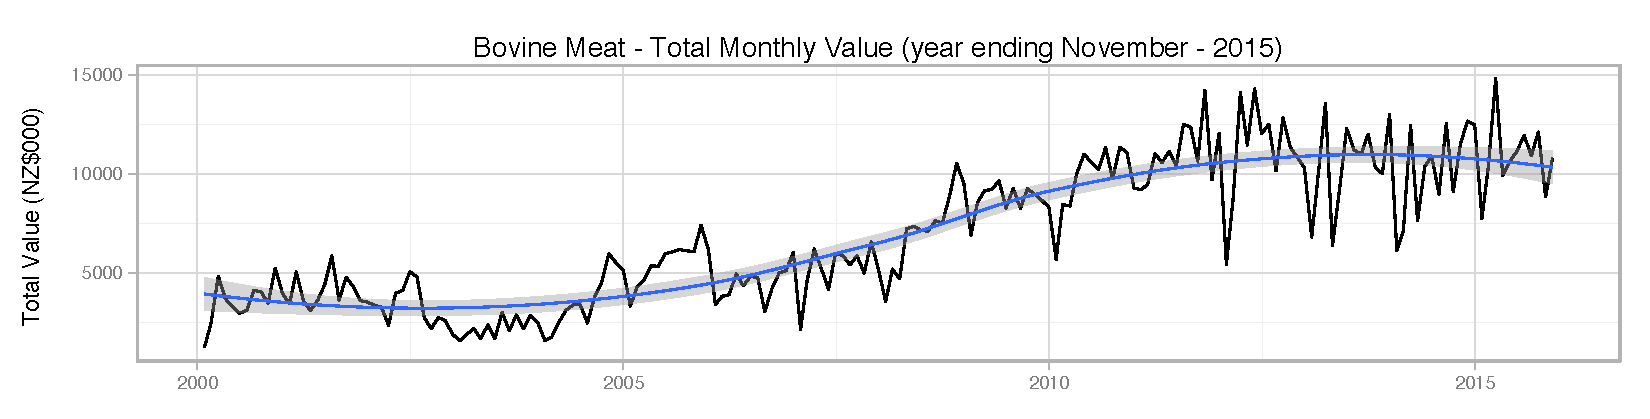
\includegraphics[scale=0.53]{../graphs/monthly_value/bovine_meat_monthly_value.pdf} \
    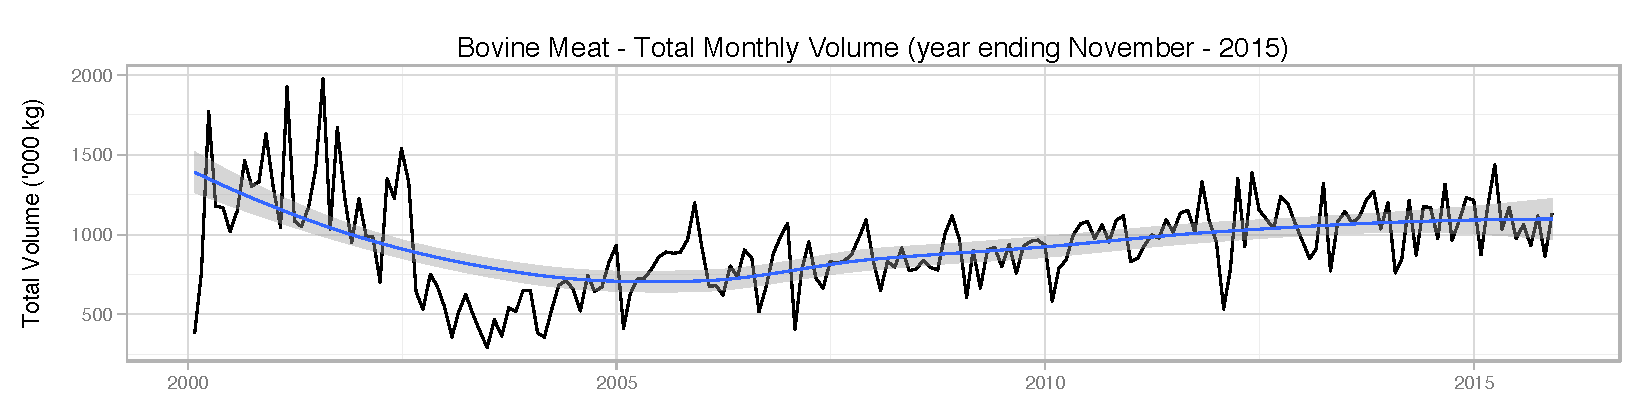
\includegraphics[scale=0.53]{../graphs/monthly_volume/bovine_meat_monthly_volume.pdf} \
    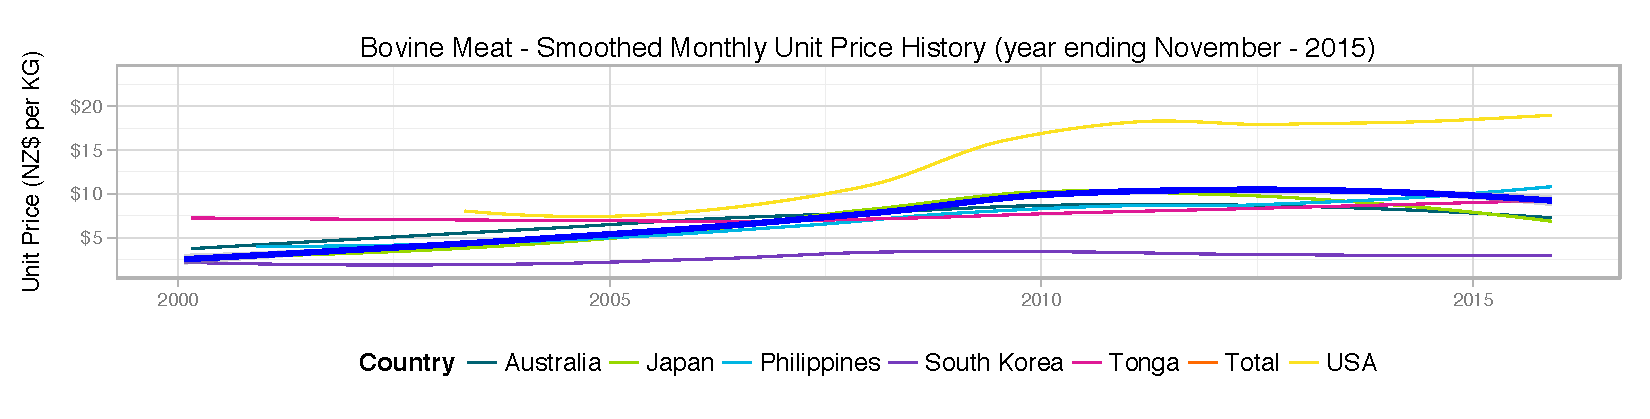
\includegraphics[scale=0.53]{../graphs/smoothed_price/bovine_meat_smoothed_price.pdf} \
    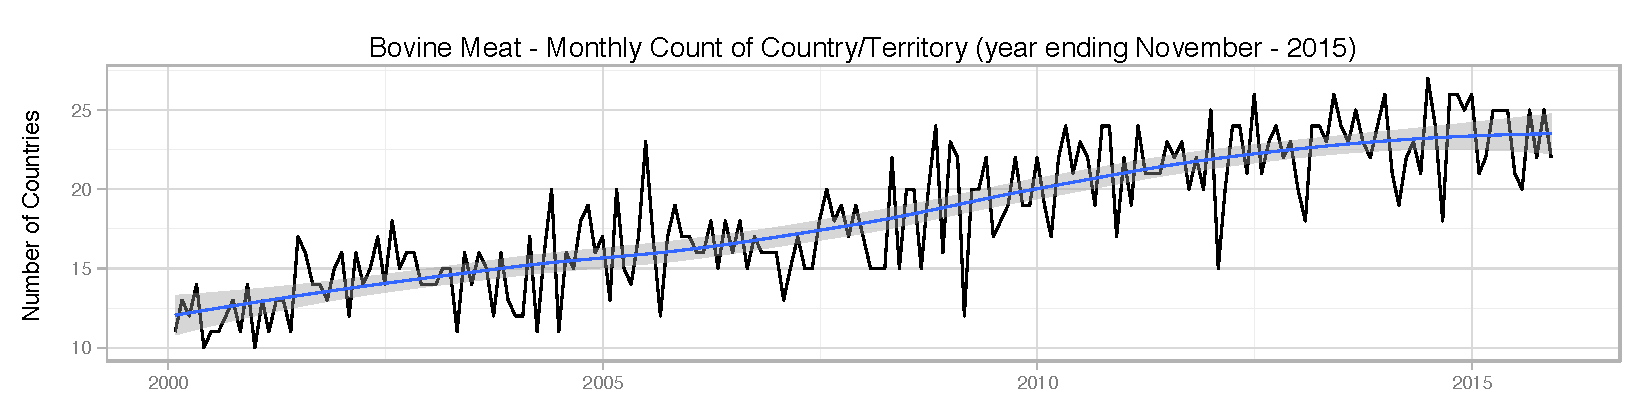
\includegraphics[scale=0.53]{../graphs/monthly_number_countries/bovine_meat_monthly_count.pdf} \
    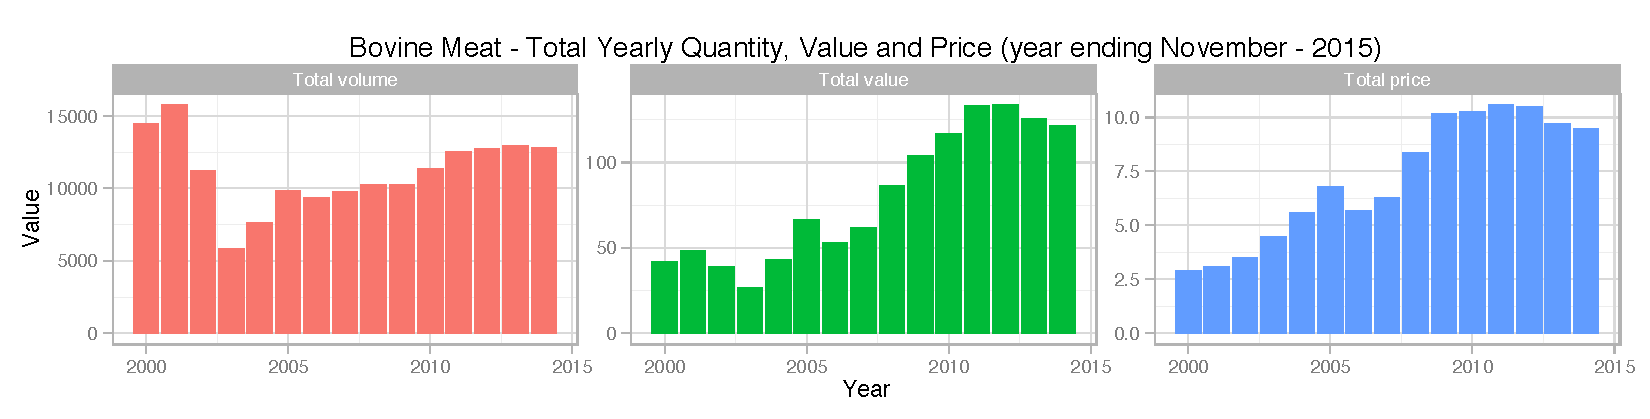
\includegraphics[scale=0.53]{../graphs/yearly_summary/bovine_meat_yearly_summary.pdf} \
   \end{figure}



\footnotetext[1]{Source: Statistics New Zealand - Overseas Merchandise Trade}
\footnotetext[2]{Harmonised System Codes for Bovine Meat starting with: 160250.}
\end{document}
